\subsection{检测效果分析}
\label{subsec:featurespy-evaluation-detection}

\paragraph*{Exp\#1(明文数据块的相似性检测)。}本文首先验证通过比较内容特征可有效地找到相似的明文数据块。本文考虑多个SYNChunk$(x, y)$数据集,每个SYNChunk$(x, y)$ 包括10\,K个从基本数据块修改得到的相似数据块($x$定义了随机修改位置的数量,$y$定义了每个修改位置处连续修改的字节数,参见\S\ref{subsec:featurespy-datasets})。 本文为 SYNChunk$(x, y)$中的每个明文数据块提取四个内容特征,如果这些数据块与基本数据块分别共享一到四个相同的特征,则认为成功识别相似数据块。本文评估每个SYNChunk$(x, y)$数据集中成功识别的与基本数据块相似的数据块占整个数据集所有数据块的比例。

\begin{figure}[!htb]
    \centering
    
\includegraphics[width=0.5\textwidth]{pic/featurespy/plot/detection/syn/fixed_pq_legend.pdf}
    \vspace{5pt}\\
    \begin{tabular}{@{\ }c@{\ }c}
        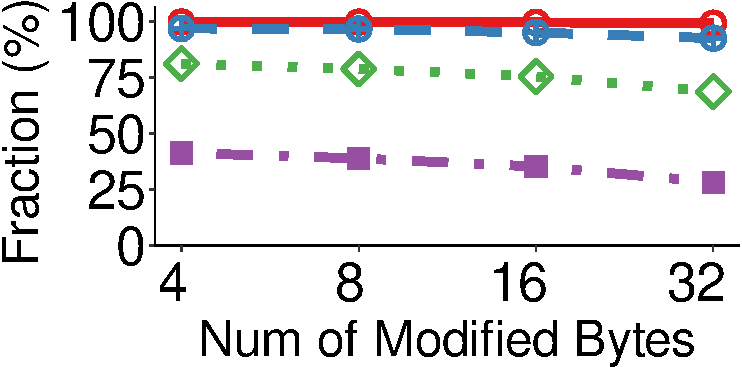
\includegraphics[width=0.45\textwidth]{pic/featurespy/plot/detection/syn/fixed_p_4.pdf} &
        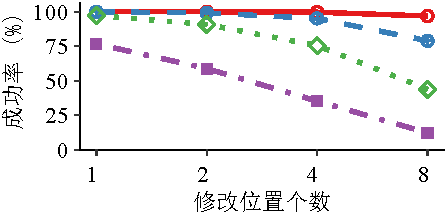
\includegraphics[width=0.45\textwidth]{pic/featurespy/plot/detection/syn/fixed_q_16.pdf}  \\
        \mbox{\small (a) 固定$x=4$,改变$y$}                                                    &
        \mbox{\small (b) 固定$y=16$,改变$x$}                                                     \\
    \end{tabular}
    \caption{(Exp\#1) 明文数据块的相似性检测}
    \label{fig:featurespy-expDetectionSynSim}
\end{figure}

图~\ref{fig:featurespy-expDetectionSynSim}(a)显示了当本文固定$x$=4并变化$y$(图~\ref{fig:featurespy-expDetectionSynSim}(a)),以及固定$y$=16并变化的$x$(图~\ref{fig:featurespy-expDetectionSynSim}(b))时产生的多个SYNChunk$(x, y)$数据集的检测结果。一般来说,识别到相似数据块的成功率随着$x$或$y$的增大而降低,这是因为修改范围越大,越有可能使数据块产生不同的内容特征。具体来说,称功率受$x$的影响比$y$更大,这是因为增加$x$将改变大量滑动窗口(\S\ref{subsec:featurespy-basic})的Rabin指纹。另一方面,本文可以通过检查数据块是否共享任意一个或两个相同的特征来有效地检测大部分(例如,至少78.9\%)的相似数据块。

\paragraph*{Exp\#2(密文数据块的相似性检测)。}
本文扩展Exp\#1来研究\sysnameF 基于密文数据块的的相似性检测能力。实验采用本文提出的相似性保留加密方法(SPE)产生密文数据块。具体来说,本文对每个明文数据块执行特征密钥生成(\S\ref{subsec:featurespy-spe}),检查为每个SYNChunk$(x, y)$中所有数据块生成的密钥相同的比例,以验证相似性保留加密为相似数据块产生相同特征密钥的能力(标记为KeyGen)。然后,本文执行SPE,使用特征密钥加密对应数据块的特征指标,并统计加密后的相似性指标与每个数据集中基本数据块的相似性指标相同的比例作为密文数据块相似性检查能力的结果。这里,本文关注三个SPE实例SPE$(1)$、SPE$(2)$和SPE$(4)$,它们将1个、2个和4个加密块(长度分别为16、32和64个字节)作为每个数据块的相似性指标。

\begin{figure*}[!htb]
    \centering
    
\includegraphics[width=0.4\textwidth]{pic/featurespy/plot/detection/syn/synBarPlotDetect_legend.pdf}\\
    \begin{tabular}{@{}c@{}c}
        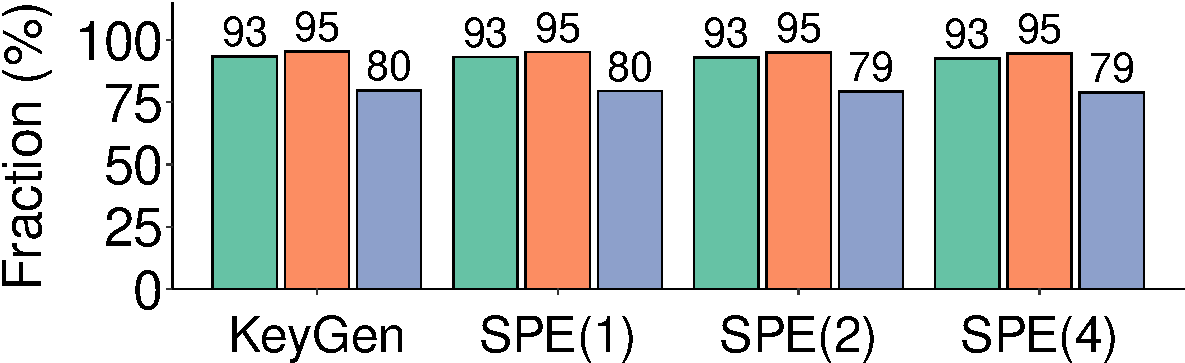
\includegraphics[width=0.49\textwidth]{pic/featurespy/plot/detection/syn/syn-p1-q4-detect.pdf}  &
        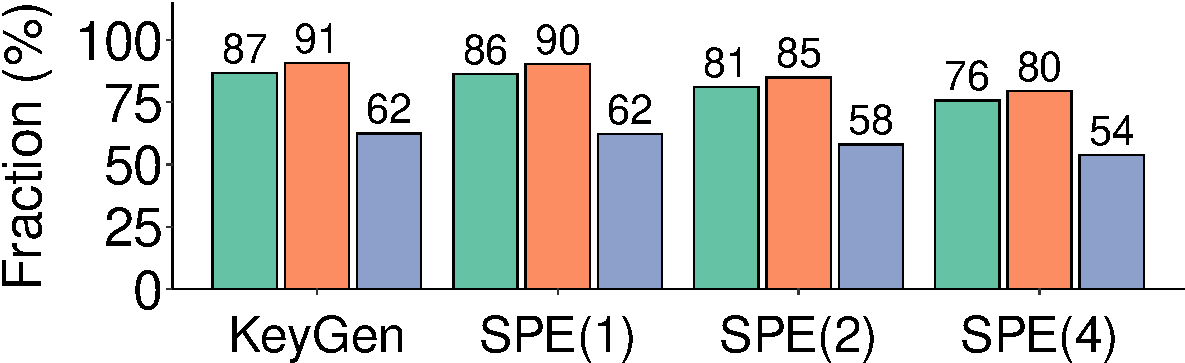
\includegraphics[width=0.49\textwidth]{pic/featurespy/plot/detection/syn/syn-p2-q8-detect.pdf}    \\
        \mbox{\small (a) $\textrm{SYNChunk}(1, 4)$}                                                     &
        \mbox{\small (b) $\textrm{SYNChunk}(2, 8)$}                                                       \\
        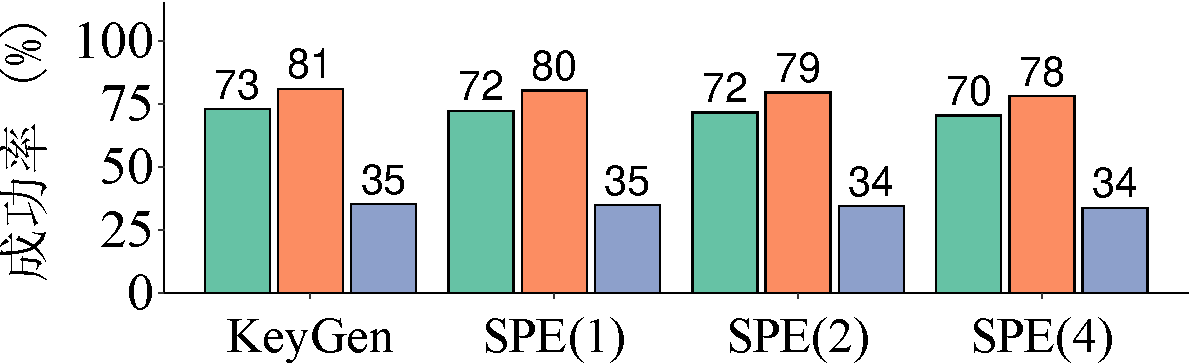
\includegraphics[width=0.49\textwidth]{pic/featurespy/plot/detection/syn/syn-p4-q16-detect.pdf} &
        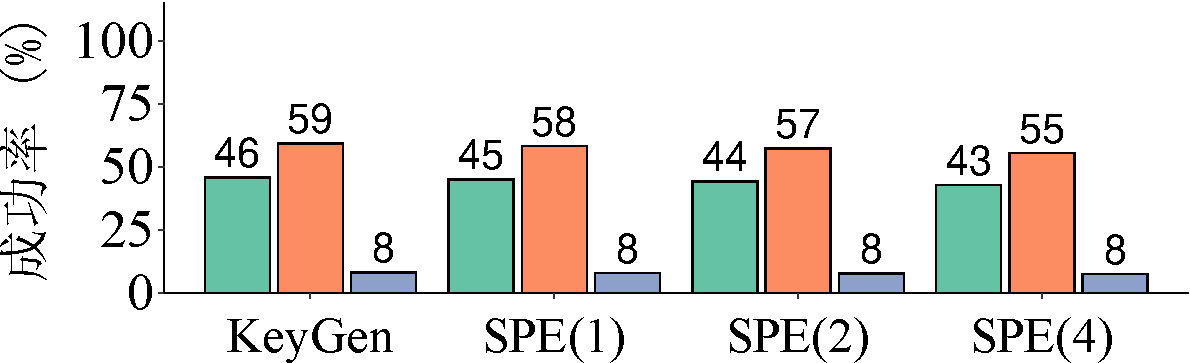
\includegraphics[width=0.49\textwidth]{pic/featurespy/plot/detection/syn/syn-p8-q32-detect.pdf}   \\
        \mbox{\small (c) $\textrm{SYNChunk}(4, 16)$}                                                    &
        \mbox{\small (d) $\textrm{SYNChunk}(8, 32)$}                                                      \\
    \end{tabular}
    \caption{(Exp\#2) 密文数据块的相似性检测}
    \label{fig:featurespy-expDetectionSynDetect}
\end{figure*}

图~\ref{fig:featurespy-expDetectionSynDetect}展示了具有最小(SYNChunk$(1,4)$)、小(SYNChunk$(2,8)$)、中(SYNChunk $(4,16)$)和大(SYNChunk$(8,32)$)差异的相似数据块产生的密文数据块的相似性检查成功率。与{\tt allFeature}相比,实例{\tt firstFeature}和{\tt minFeature}为仅为更相似的数据块生成相同的特征密钥,尤其是当修改量很大时。例如,{\tt firstFeature}和{\tt minFeature}分别为45.7\%和59.3\%的数据块产生相同密钥,但{\tt allFeature}仅为8.1\%的数据块生成了相同特征密钥。此外,{\tt minFeature}为差异较大的相似数据块产生相同特征密钥的能力优于{\tt firstFeature},这可能是因为最小内容特征对数据块内容的随机变化更不敏感。此外,本文观察到相似性保留加密在加密后保留了较高的相似性。具体来说,通过检查密文数据块中的相似性指标,本文在SYNChunk$(1,4)$、SYNChunk$(2,8)$、SYNChunk$(4,16)$和SYNChunk$(8,32)$,分别检测到至多95.2\%、90.4\%、80.2\%和58.3\%的相似数据块。

\paragraph*{Exp\#3(推测内容攻击检测案例研究)。}
本文扩展了\S\ref{sec:featurespy-attack}中的案例研究,以研究 \sysnameF 如何检测推断工资和签约奖金的推测内容攻击。本文用一个固定报告阈值$T$=3\%和一个大小为两个加密块(等效32字节)的相似性指标来配置 \sysnameF。参考\S\ref{sec:featurespy-attack},攻击者需要伪造101$\times$31=3131个文件,其中年薪和签约奖金分别有101和31个可能值。为了模拟在正常数据集中混合伪造文件(否则更容易被检测到)的攻击者,本文将所有伪造文件随机插入到每个Linux/CouchDB(由于FSL和MS数据集不含实际数据,因此不予考虑)快照中的文件之间,并对每个快照中的文件(及伪造的文件)单独执行数据分块\cite{fsl, meyer2011deduplication},并在产生的数据块之上应用相似性保留加密。本文以检测率(\sysnameF 成功检测到的此类攻击快照的数量与使用的快照总数的比率)作为评价标准。此外,本文使用\sysnameF 处理每个原始快照中的所有文件(不包含伪造的文件),评估\sysnameF 的误判率(即\sysnameF 误判的快照数量与原始快照总数的比率)。本文展示了\sysnameF 如何检测推测内容攻击,并给出整体的检测结果。

\begin{figure*}[!htb]
    \centering
    
\includegraphics[width=0.8\textwidth]{pic/featurespy/plot/detection/overall/prefixDistribution_legend.pdf}\\
    \begin{tabular}{cc}
        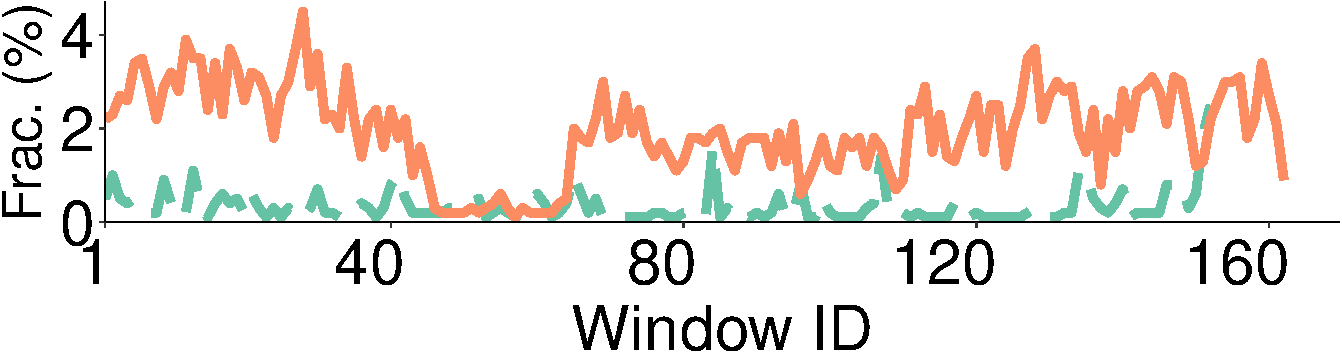
\includegraphics[width=0.472\textwidth]{pic/featurespy/plot/detection/overall/prefixDistribution-1000-Linux-first.pdf} &
        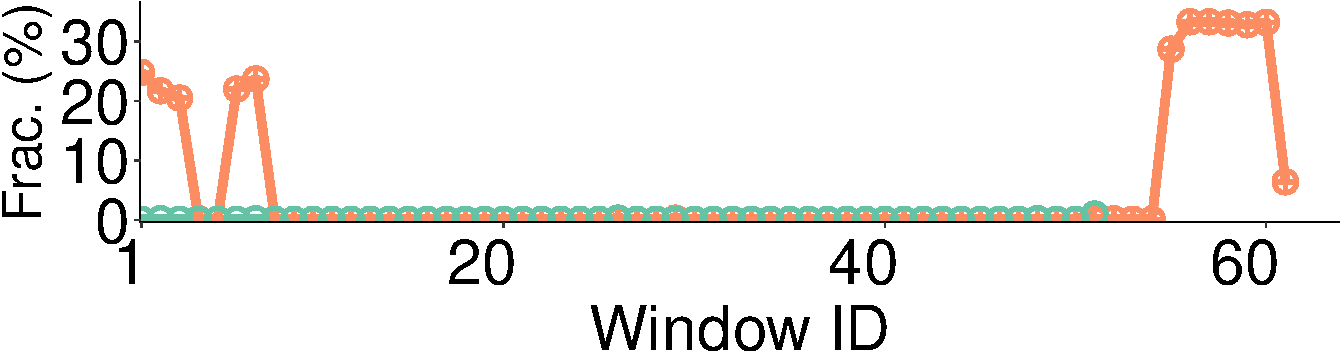
\includegraphics[width=0.472\textwidth]{pic/featurespy/plot/detection/overall/prefixDistribution-1000-CouchDB-first.pdf} \\
        \mbox{\makecell[c]{\small (a) {\tt Linux:firstFeature}实例}}                                                           &
        \mbox{\makecell[c]{\small (b) {\tt CouchDB:firstFeature}实例}}                                                           \\        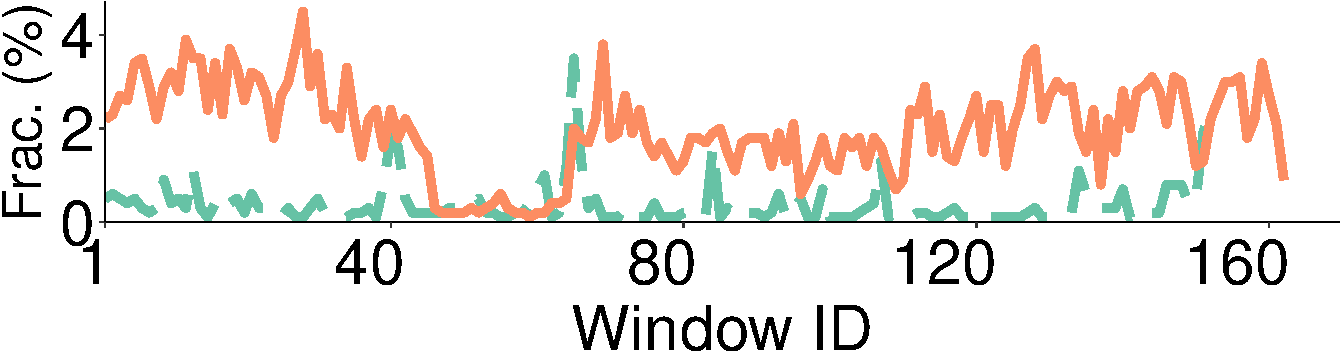
\includegraphics[width=0.472\textwidth]{pic/featurespy/plot/detection/overall/prefixDistribution-1000-Linux-min.pdf} &
        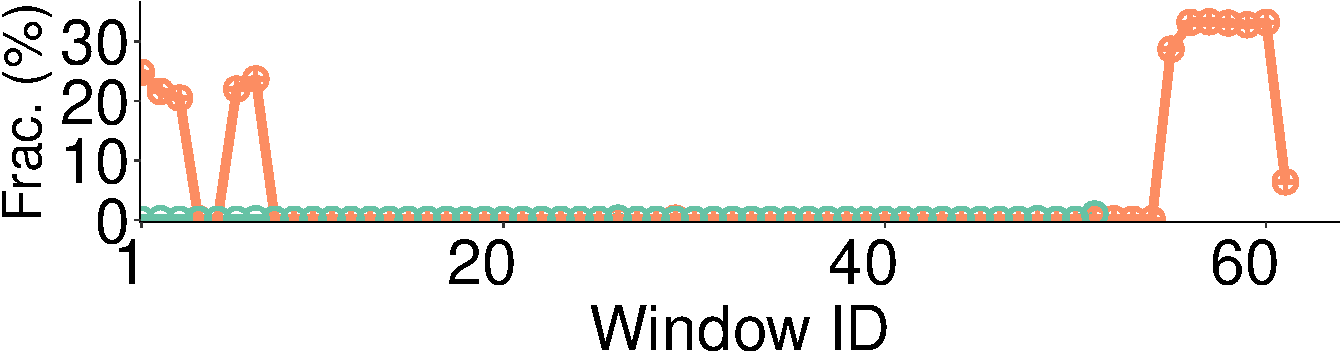
\includegraphics[width=0.472\textwidth]{pic/featurespy/plot/detection/overall/prefixDistribution-1000-CouchDB-min.pdf}   \\
        \mbox{\makecell[c]{\small (c) {\tt Linux:minFeature}实例}}                                                             &
        \mbox{\makecell[c]{\small (d) {\tt CouchDB:minFeature}实例}}                                                             \\
        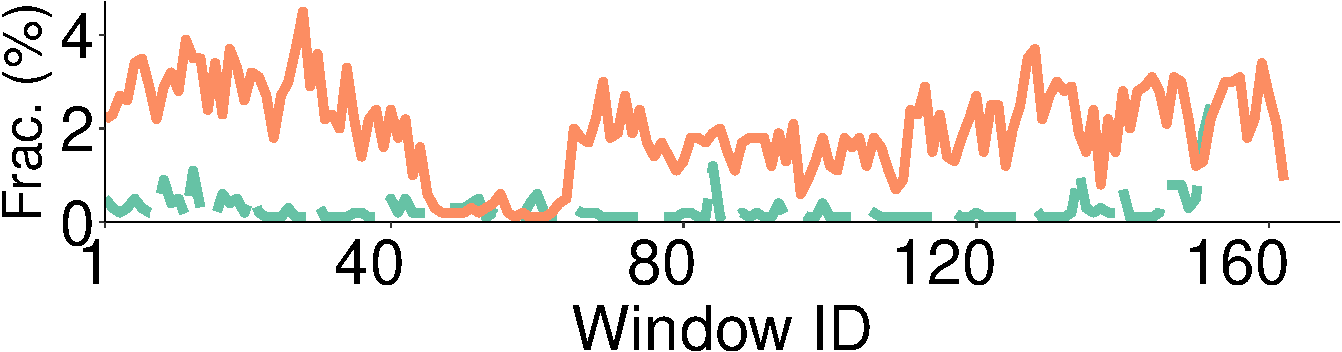
\includegraphics[width=0.472\textwidth]{pic/featurespy/plot/detection/overall/prefixDistribution-1000-Linux-all.pdf}   &
        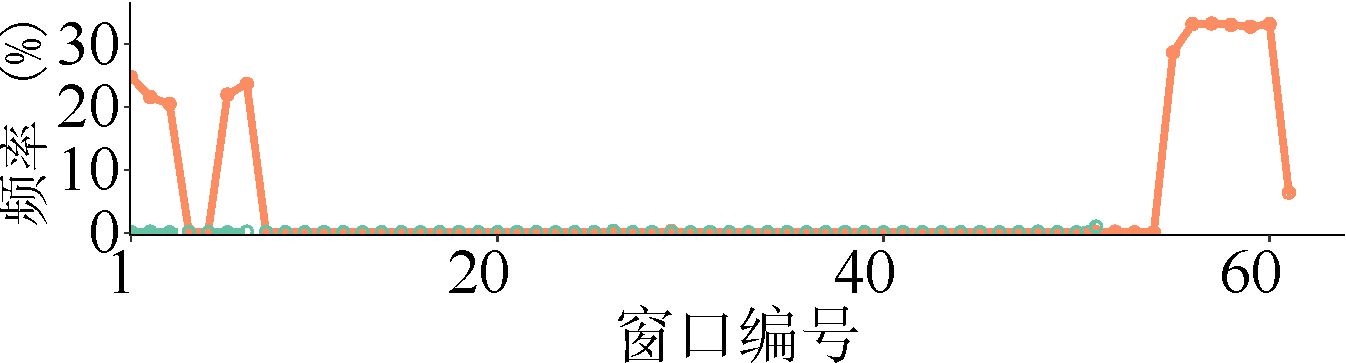
\includegraphics[width=0.472\textwidth]{pic/featurespy/plot/detection/overall/prefixDistribution-1000-CouchDB-all.pdf}   \\
        \mbox{\makecell[c]{\small (e) {\tt Linux:allFeature}实例}}                                                             &
        \mbox{\makecell[c]{\small (f) {\tt CouchDB:allFeature}实例}}                                                             \\
    \end{tabular}
    \caption{(Exp\#3)攻击检测示例:给出了使用{\tt firstFeature}、{\tt minFeature}和{\tt allFeature}方案分别处理包含伪造文件(即攻击,Attack)和不包含伪造文件(即不发生攻击,Raw)的Linux/CouchDB最后一个版本的快照时每个窗口(大小固定为$W$=1\,K)中最高频相似性指标的出现频率。}
    \label{fig:featurespy-expDetectionOverall}
\end{figure*}

图~\ref{fig:featurespy-expDetectionOverall}显示了\sysnameF 的三种实例在检测原始Linux快照(v5.13)和CouchDB快照(v6.6.2)以及插入伪造文件后的快照时的结果。具体来说,x轴为处理窗口(大小固定为$W$=1\,K)的顺序编号,y轴为每个窗口中具有相同相似性指标的数据块占该窗口中所有数据块的比例。本文观察到所有三个实例都可以有效地检测到推测内容攻击,因为它们在攻击快照(Attack)中至少有一个窗口的最高频率超过了阈值$T$=3\%(即,具有相同相似性指标的密文数据块的比例大于$T$=3\%)。另一方面,{\tt minFeature}方案在Linux快照中发生了误判,这是由于其至少有一个正常的窗口(例如,Raw的第65个窗口)中,具有相同相似性指标的密文数据块的比例大于阈值$T$=3\%。

\begin{figure}[!htb]
    \centering
    
\includegraphics[width=0.5\textwidth]{pic/featurespy/plot/detection/overall/effectiveness-falsePositive_legend.pdf}
    \vspace{5pt}\\
    \begin{tabular}{@{\ }c@{\ }c}
        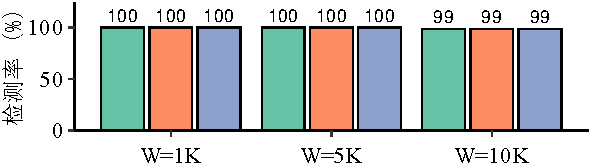
\includegraphics[width=0.6\textwidth]{pic/featurespy/plot/detection/overall/effectivenessLinux.pdf} &
        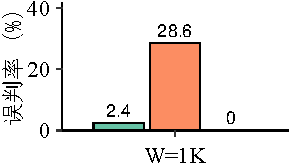
\includegraphics[width=0.3\textwidth]{pic/featurespy/plot/detection/overall/falsePositiveLinux.pdf}   \\
        \mbox{\small (a) 检测率}                                                                            &
        \mbox{\small (b) 误判率}                                                                              \\
    \end{tabular}
    \caption{(Exp\#3) 每个Linux/CouchDB快照中的总体检测率和误判率}
    \label{fig:featurespy-expDetectionOverallFalsePositive}
\end{figure}

图~\ref{fig:featurespy-expDetectionOverallFalsePositive}显示了本文将\sysnameF 的检测窗口大小分别配置为1\,K,5\,K和10\,K时Linux数据集中的总体检测率和误判率。在各个窗口大小设置下,\sysnameF 均实现了很高的检测率(例如,至少98.6\%)。然而,较大的窗口会略微降低检测率,这是因为大窗口中仅有相对较小部分的密文数据块具有相同的相似性指标。此外,\sysnameF 仅在窗口大小为1\,K时才会产生误判(图~\ref{fig:featurespy-featureDistribution}(b)),这是因为原始快照(Raw)当中本身包含较多的相似数据块。但即使在这种情况下,{\tt allFeature}也没有任何误判,这是因为它只能检测到少量相似度较高的数据块。另一方面,可检测到更多相似数据块(Exp\#2)的{\tt minFeature}方案会产生28.6\%的误判。

除了Linux数据集,本文也在CouchDB数据集中评估\sysnameF,并发现所有\sysnameF 的实例均可成功检测到所有混合在CouchDB数据集的快照中的推测内容攻击(即具有100\%的检测率),且没有引入任何误判。可能的原因是每个 CouchDB快照中几乎不含有相似数据块,当注入许多对伪造文件产生的相似数据块时,\sysnameF 可以立即检测到(相似数据块的)频率分布变化。

%TODO
\paragraph*{Exp\#4(目标文件熵对攻击检测的影响)。}

本文扩展研究\sysnameF 在检测具有特定信息熵的目标文件时的检测率,即针对具有不同信息熵的目标文件SYNFile$(x, y)$($x$是文件中未知变量的数量,$y$是每个变量的可能取值的数量,参见\S\ref{subsec:featurespy-datasets})的检测能力。本文枚举了目标文件的$x\times y$个可能值,将它们随机插入到Linux数据集最后一个快照(v5.13,大小为985.9\,MiB)包含的文件序列中,并评估100次随机生成的目标文件数据集下\sysnameF 的检测率(阈值设置为固定的$T$=3\%)。

\begin{figure}[!htb]
    \centering
    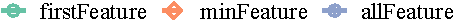
\includegraphics[width=0.5\textwidth]{pic/featurespy/plot/detection/trade-off/trade_off_legend.pdf}
    \vspace{5pt} \\
    \begin{tabular}{@{\ }c@{\ }c@{\ }c}
        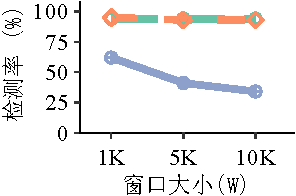
\includegraphics[width=0.32\textwidth]{pic/featurespy/plot/detection/trade-off/varyWindow_linux.pdf}    &
        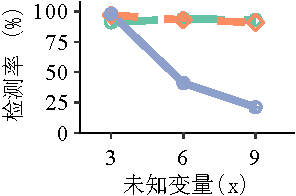
\includegraphics[width=0.32\textwidth]{pic/featurespy/plot/detection/trade-off/varyModifyPos_linux.pdf} &
        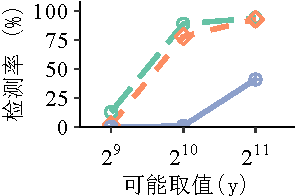
\includegraphics[width=0.32\textwidth]{pic/featurespy/plot/detection/trade-off/varyFileNumber_linux.pdf}  \\
        \makecell[c]{\small (a) 改变窗口大小$W$                                                                   \\ \small 检测SYNFile$(6,2048)$数据集} &
        \makecell[c]{\small (b) 固定窗口大小$W$=5\,K                                                              \\ \small 检测SYNFile$(\cdot,2048)$数据集} &
        \makecell[c]{\small (c) 固定窗口大小$W$=5\,K                                                              \\ \small 检测SYNFile$(6,\cdot)$数据集} \\
    \end{tabular}
    \caption{(Exp\#4)针对不同伪造文件集合的检测率}
    \label{fig:featurespy-expDetectionTradeOff}
\end{figure}

图~\ref{fig:featurespy-expDetectionTradeOff}(a)展示了当改变窗口大小$W$时检测到对SYNFile$(6,2048)$目标文件的攻击的检测率结果。{\tt firstFeature}和{\tt minFeature}的检测率基本不受到窗口大小$W$的影响(例如,始终保持在93\%以上),但{\tt allFeature}的检测率随着窗口大小增大而下降到34\%。其原因是{\tt allFeature}只能检测到少量相似度较高的数据块(Exp\#2),当窗口大小$W$很大时,这些数据块在窗口内的占比很低。图~\ref{fig:featurespy-expDetectionTradeOff}(b)展示了改变目标文件中未知变量$x$的数量时的检测结果。本文观察到,当$x$=9时,{\tt allFeature}的检测率再次急剧下降到21\%,这是因为它无法检测到具有更多差异区域的相似数据块。

图~\ref{fig:featurespy-expDetectionTradeOff}(c)展示了当改变目标文件中每个变量的可能值的数量$y$时的结果。当$y$为512时,所有三个实例的检测率都较低(例如,仅为13\%)。其原因是目标文件的信息熵较低,攻击者只需要构建少量相似的内容,导致\sysnameF 难以在混在的数据块流中找到相似数据块。一种可能的解决方案是配置一个较小的阈值$T$或窗口大小$W$以在检测到少数几个相似数据块时报告攻击行为,但这会增加在不同工作负载中误判的可能性。对此,本文提出了一项未来的研究方向,即如何自动平衡检测对低信息熵文件的攻击和在处理不同工作负载时最大限度地减少误判之间的权衡。